%\documentclass[handout]{beamer}
\documentclass{beamer}

\usepackage[english]{babel}
\usepackage[latin1]{inputenc}
\usepackage{textpos}
\usepackage{epstopdf}
\epstopdfsetup{update}
%\usepackage{pgfpages}
%\pgfpagesuselayout{resize to}[letterpaper,landscape]
%\usepackage{epstopdf}
%\epstopdfsetup{update}
\usepackage{pgfplots}
\usepackage{pgfbaseimage}
\usepackage{amsmath} 						%More mathematical
\usepackage{multirow}
%\usepackage[absolute,overlay]{textpos}
%\usepackage[tikz]{bclogo}
%\usepackage{etoolbox}
% listings for matlab code:
\usepackage{listings}
%\usepackage[autolinebreaks, useliterate]{mcode}
\lstset{backgroundcolor=\color[gray]{0.9}}

\usepackage{chemplants}
\usepackage{cancel}
\usepackage{graphicx}
\usetikzlibrary{math}
\usepackage{wasysym}
\usepackage{marvosym}

\usepackage{animate}

\usetikzlibrary{shapes.arrows}
\tikzset{My Arrow Style/.style={single arrow, draw=green!40!gray, very thick, fill=green!20!gray!10, anchor=base, align=center,text width=2cm,text=green!40!gray,rotate=-90,minimum width=0.5cm, inner sep=1mm, minimum height=0.5cm}}
\newcommand{\MyArrow}[2][]{\tikz[baseline] \node [My Arrow Style,#1] {#2};}

%-------------------------------------------------
% FOOTER
%
% Choose your footer style, by commenting other options:
%
%% - Clean: no footer, except of page number
\mode<presentation>{\usetheme{presentationTemplateBiomathFClean}}
%%  - Info: a fixed footer with basic presenter information
%\mode<presentation>{\usetheme{presentationTemplateBiomathFInfo}}
%%  - Section: Provide the sections and current section in the footer 
%\mode<presentation>{\usetheme{presentationTemplateBiomathFSection}}
%-------------------------------------------------


%voor de hand-outs
%\usepackage{pgfpages}
%\pgfpagesuselayout{2 on 1}[a4paper,border shrink=5mm]

\title{\LARGE Modelling and Simulation \normalsize of Biosystems}
\title{Modelling and Simulation of Biosystems}
\author[Daniel Illana]{Daniel Illana Gonz\'alez} %(daniel.illanagonzalez@ugent.be)}
\subtitle{Practicum 6: Sensitivity and uncertainty}
\date{Academic year 2024-2025}


\newcommand{\mtx}[2]
  {\left[\begin{array}{#1}#2\end{array}\right]}
\newcommand{\eqset}[1]
  {\left\{\begin{array}{rcl}#1\end{array}\right.}
\newcommand{\rbar}[2]
  {\left.#1\right|_{#2}}
\newcommand{\atwp}[1]
  {\rbar{#1}{\overline{X},\overline{U}}}

\usepackage{mdframed}

\newenvironment{opgave}[2][]{%
	\mdfsetup{%
		frametitle={%
			\tikz[baseline=(current bounding box.east),outer sep=0pt]
			\node[anchor=east,rectangle,fill=gray!40]
			{\strut #1};}%
	}
	\mdfsetup{%
		innertopmargin=10pt,linecolor=white!30,%
		linewidth=0pt,topline=true,%
		frametitleaboveskip=\dimexpr-\ht\strutbox\relax%
	}
	
	\begin{mdframed}[]\relax}{%
\end{mdframed}}



% Table of contents at the beginning of each section
%\AtBeginSection[]
%{
%  \begin{frame}
%    \frametitle{Outline}
%    \tableofcontents[currentsection]
%  \end{frame}
%}

% Title page customisation
\titlegraphic{}

\begin{document}

\frame[plain]{\titlepage}


\frame{
\frametitle{Pluto notebooks}
\large

Download the exercise notebooks for today. \vfill

\begin{itemize}
\item For this practicum, go to the Ufora submodule\\ \textbf{P6: SensUncert $>$ files} \vfill
\item Download the Pluto notebooks and put them into your dedicated \texttt{modsim\_practica/P6\_sensi} folder. \vfill
\item Go to your dedicated folder (cf. \texttt{modsim\_practica}) with a \textit{File Explorer}, then in this location either \vfill
\begin{itemize}
\item right click on your mouse and choose \texttt{Open in Terminal} (or something alike), or
\item write the command \texttt{cmd} in the address bar and click [\textit{Enter}].
\end{itemize} \vfill
\item Execute \texttt{julia launch\_pluto.jl} \vfill
\item Now you will be able to open and run the Pluto notebook of you choice. \vfill
\end{itemize}
}


\frame{
\frametitle{Today}
\Large
\begin{itemize}
	\item Local sensitivity analysis (LSA) \medskip
%	\begin{itemize}
%	\item Local sensitivity analysis (LSA)
%	\end{itemize}
	\item Uncertainty analysis (UA) \bigskip

	\item Examples (intro notebooks)
	\begin{itemize}
		\large
		\item Logistic growth model
	\end{itemize} 
	\bigskip
	\item Exercises %to do 
	\begin{enumerate}
		\large
		\item Exponential + Gompertz growth model (intro notebooks)
		\item Fermenter - Monod kinetics
		\item Bitrophic model
		\item Insuline model (sensitivity only)
	\end{enumerate}
\end{itemize}
}


\frame{
  \frametitle{Goals of this practicum}
  \Large \bigskip
  \color{beamerstructure}
  {\begin{enumerate}
	\item Calculating and interpreting local sensitivity \medskip
	\item Calculating the variability in the output due to uncertainty in model parameters
  \end{enumerate}
  }

\bigskip \bigskip %\pause

\large
The following notebooks are the subjects for today:\medskip
\begin{itemize}
\item \texttt{sens\_intro.jl} (introduction) \medskip
\item \texttt{sens\_fermenter\_monod.jl}
\item \texttt{sens\_bitrophic\_model.jl} 
\item \texttt{sens\_insuline.jl} (extra) \bigskip
\item \texttt{uncert\_intro.jl} (introduction) \medskip
\item \texttt{uncert\_fermenter\_monod.jl}
\item \texttt{uncert\_bitrophic\_model.jl} \bigskip
\end{itemize}
}


\frame{
\frametitle{Local sensitivity analysis}
\large\medskip
`\textit{How sensitive is the model output to changes in parameter values?}'

\bigskip


When the model output is highly \textbf{sensitive} to a certain parameter, \textit{\color{ugent-la}small} changes in the value of this parameter have a \textit{\alert {large}} impact or influence on the value of the model output.

\bigskip \pause

Mathematically, the sensitivity of output $\hat{y}_i$ on the parameter $\theta_j$ is:

$$
S_{ij} = \cfrac{\partial \hat{y}_i(\theta)}{\partial \theta_j}
$$

\begin{itemize}
\item How sensitive output $\hat y_i$ is to changes in parameter $\theta_j$. \smallskip
\item \textit{Local} sensitivity thus depends on the value of parameter  $\theta_j$. \smallskip
\item $S_{ij}$ is also called the \textit{absolute} sensitivity function (cf. see next).
\end{itemize}

}


\frame{
\frametitle{Local sensitivity analysis}
\large \bigskip

Usually, a numerical approximation is needed:

$$
\cfrac{\partial \hat{y}_i(\theta)}{\partial \theta_j} \approx \cfrac{\hat{y}_i(\theta_j+\Delta\theta_j)-\hat{y}_i(\theta_j)}{\Delta\theta_j}
$$

\begin{itemize}
\item The model is evaluated for $\theta_j$ and $\theta_j+\Delta\theta_j$. \medskip
\item Dependent on the units of $\hat{y}_i$ and $\theta_j$ !
\end{itemize}

\bigskip \pause

A \textit{normalized} variant exists, also called (\textit{total}) \textit{relative} sensitivity:

$$
S_{ij, rel} = \cfrac{\partial \hat{y}_i(\theta)}{\partial \theta_j} \cdot \cfrac{\theta_j}{\hat{y}_i}
$$

\begin{itemize}
\item Percentage of change in the output $\hat{y}_i$ for a one per cent of change in the parameter value $\theta_j$. Units no longer relevant. \bigskip
\item Can be used for comparison for different parameters/variables.
\end{itemize}


}




\frame{
\frametitle{In practice}
\large

\texttt{using {\color{ugent-la}ForwardDiff}}

\bigskip

\texttt{function solution(params)}\\
\qquad \texttt{$\theta_1$, $\theta_2$, ... = params}\\
\qquad \texttt{u0 = [:y1=>..., :y2=>...]}\\
\qquad \texttt{tspan = (..., ...)}\\
\qquad \texttt{oprob = ODEProblem(...)}\\
\qquad \texttt{osol = solve(...)}\\
\qquad \texttt{return osol}\\
\texttt{end}\\

\bigskip

\texttt{output\_yi(params) = solution(params)[:yi]}\\

\bigskip

\texttt{yi = output\_yi(\texttt{$\theta_1$,$\theta_2$,...})}\\

\bigskip

\texttt{sens\_yi = {\color{ugent-la}ForwardDiff.jacobian}(output\_yi,[$\theta_1$,$\theta_2$,...])}\\

\bigskip

\texttt{sens\_yi\_$\theta_j$\_rel = sens\_yi[:,j] .* $\theta_j$ ./ yi}

}

\frame{
\frametitle{In practice}
\large\bigskip

\centering
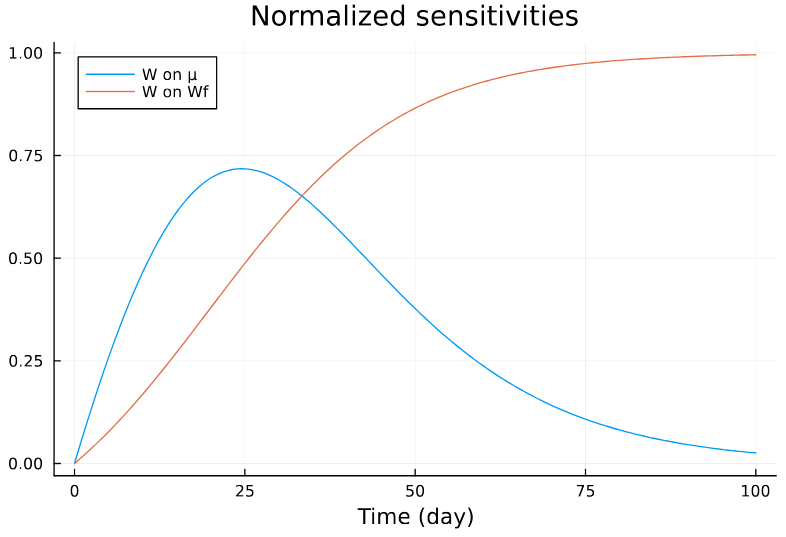
\includegraphics[width=0.9\linewidth]{figs/sensitivity_fig_example.png}

\normalsize \medskip

Task: \textbf{find out which parameters affect output the most} 

}


\frame{
\frametitle{Uncertainty analysis}
\large

Parameters are rarely known with absolute certainty, due to e.g.: \medskip
\begin{itemize}
\item measurement errors
\item variability in real-world conditions
\item incomplete knowledge about the system
\end{itemize}

\bigskip

Uncertainty can \textit{propagate} through the model equations, leading to uncertainties in the outcomes predicted by the model. 
Performing an \textbf{uncertainty analysis can thus increase the reliability} of our models and help us detect flaws or overconfidence in their results.

\bigskip\bigskip

Both sensitivity and uncertainty analyses are powerful methods in the toolbox of modelers. You can also apply them to your projects!

}



\frame{
\frametitle{In practice}
\large

\texttt{using {\color{ugent-la}Measurements}}

\medskip

\texttt{params = [:$\theta_1$=>value1{\color{ugent-la}$\,\pm\,$std1}, :$\theta_2$=>value2{\color{ugent-la}$\,\pm\,$std2}, ...]}

\bigskip

%The rest is identical as in ODE1/ODE2.

\centering
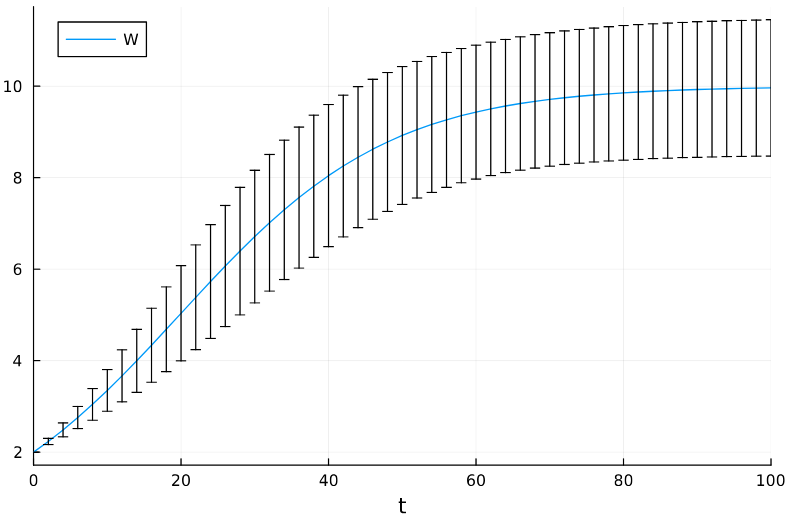
\includegraphics[width=0.8\linewidth]{figs/uncertainty_fig_example.png}

\normalsize \medskip

Task: \textbf{quantify how parameter uncertainty propagates }

}


\end{document}

